\chapter{Methods}\label{methods}

\section {Participants and stimuli}

\subsection{Participants}

18 children and 22 adults were recruited from the internal participants database.
Subjects were selected if they spoke German as native language, if their language development was unremarkable, if their handedness score was above 70, if they fulfilled the prerequisites for MRI scans, and if their medical history was free of cognitive abnormalities.
4 children and 4 adults dropped out inbetween sessions of the study.
Two children were excluded from the analysis because their behavioral performance was at chance level.
12 children (5 female) and 18 adults (9 female) were left for the subsequent analysis.
Children were aged between 9y11m and 10y9m and described as right-handed by their parents.
Adults were aged between 22 and 33 years and scored between 73 to 100 (median: 95) on the laterality quotient test \cite{3.1.LQ}.
The point of reference for these ages is the time of the MEG session.
Parents gave written informed consent and were compensated with 40\euro \ for the MEG session and 7,50\euro \ for the MRI session.
Children agreed to participate in the study and were compensated with a 10\euro \ gift voucher for each session.
Adult participants were compensated with 20\euro.
All experimental procedures were approved by the University of Leipzig Ethical Review Board.


\subsection{Task}

The study consisted of two sessions: an anatomical MRI acquisition (duration: 50 minutes) and an interactive magnetoencephalographic measurement (typical duration: 90 minutes).
Since they took place in two different locations, there was a delay (median: 98 days, maximum: 243 days) between the two sessions.

The MRI session is described in detail in section 3.2.2.

The MEG session consisted of two sections: a tutorial section and a main section.

\paragraph{MEG tutorial section}

First, the tutorial section described the usage of the interface.

Second, subjects needed to respond to an example stimulus with the spoken sentence written out below the screen.

Third, three example trials followed without the written sentence.

Fourth, an artificially incomprehensible sentence was presented together with otherwise innocuous visual stimuli.

When subjects pressed either response button instead of skipping the trial, they were instructed with the skip function.

Finally, a series of randomized tutorial trials followed.
When subjects showed behavioral proficiency of the task, the tutorial ended prematurely.
Two thresholds for proficiency were possible: either an average response time below 3000ms and an accuracy score above 80\%, or an accuracy score above 88\%.
Either threshold could only be reached after completing at least 5 or 8 trials, respectively.
When none of these thresholds were met, the tutorial ended after 36 trials.

\paragraph{MEG main section}
The main section was used for MEG acquisition and consisted of 304 trials grouped in two blocks.
There was a scheduled break between the blocks (usually 1-2 minutes) which included interaction with the research assistant.
Subject-specific trial randomization was performed before the task.
All stimuli-related randomization tasks were implemented with a time-seeded Mersenne-Twister approach in Python 2.7.
Randomization contained two exceptions: neither the same image nor the same sentence could be played twice in a row.
Each block consisted of 8 clusters.
Subjects were shown a feedback screen at the end of each cluster, summarizing their performance throughout the recent cluster.
Since manual intervention was necessary to proceed to the next cluster, subjects frequently used this opportunity for a tiny break (typically 5-20 seconds).
Each cluster consisted of 19 trials.

\paragraph{Structure of a single trial}
Each trial started by showing two pictures side-by-side.
In one picture, one of the animals performs a social action on the other animal.
In the other picture, the roles are reversed.
10ms later, the spoken question started playing.
The subject could respond by pressing one of the direction buttons or the skip button.
There were two direction buttons, left or right, signifying that the left or right image contained the answer to the question.
The skip button was used to mark the trial as invalid for further analysis, and excluded the trial from performance feedback.
This response was the correct choice when the subject was distracted or failed to comprehend the question immediately.
This opened a minor pitfall: subjects could have gotten perfect scores by just pressing the skip button each time.
Fortunately, none of the subjects discovered this opportunity.
The trial ended with an auditory and visual feedback.


\subsection{Visual stimuli}

\paragraph{Character motivation}
A set of visual stimuli consisted of a two side-by-side images on black background.
Each image depicted two different animals on a white background.
I selected selected social activities that were only plausible for antropomorphised characters, not for their real animal counterparts.
Antropomorphization includes the use of their front limbs for object manipulation and standing on their hindlegs.
These measures are introduced to prevent associations with real-world animalistic behavior.
For example, a lion "'catching"' a monkey could resemble predatory behavior.
This association with chasing and killing would introduce a semantic bias against the reverse interaction: a real-life monkey "'catching"' a lion is much more implausible than the reverse.
To further detract from a naturalistic view, the animals were represented in a cartoon style.
To prevent unnecessary stress on this interpretation, I only selected animals whose real-life counterparts were approximately equally sized.

\begin{figure}[h]
\begin{center}
\vspace{7mm}
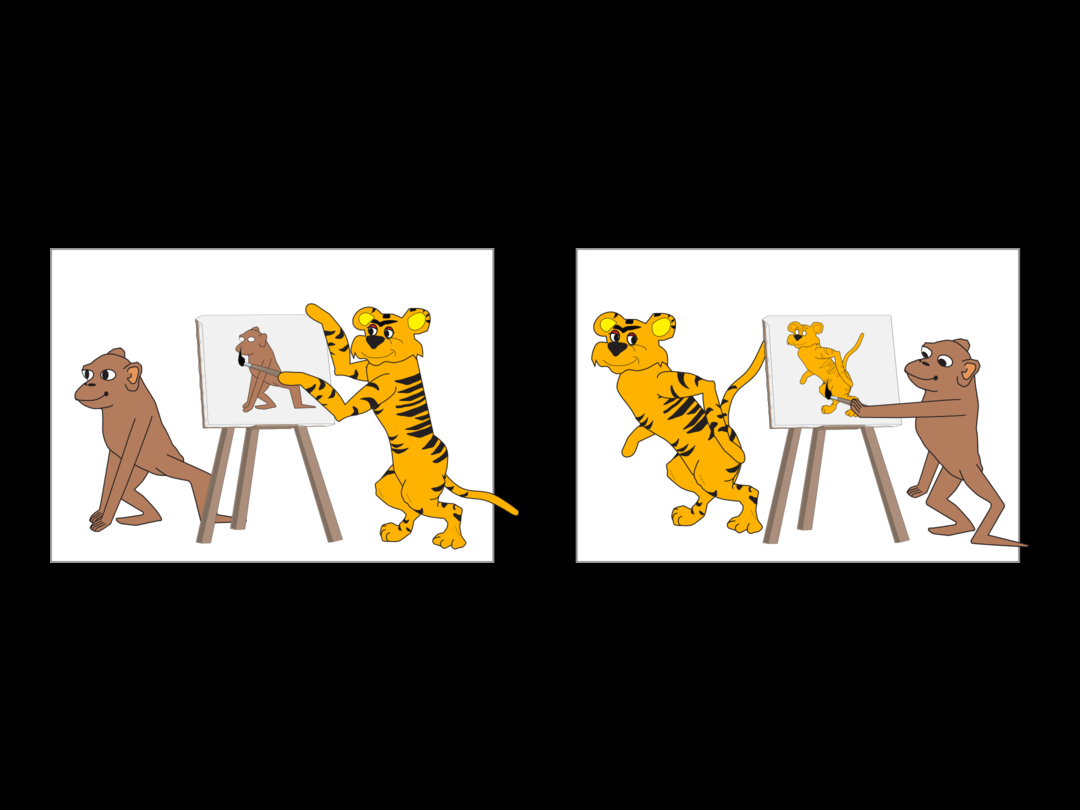
\includegraphics[width=0.5\textwidth]{pics/3_1_screen}
\caption{\label{3.1.screen} A typical visual stimulus, featuring two pairs of animals.}
\end{center}
\end{figure}

Image components were adapted with permission and kind advice from \cite{3.1.animals}.
Modifications were performed with Inkscape.

\begin{figure}[h]
\begin{center}
\vspace{7mm}
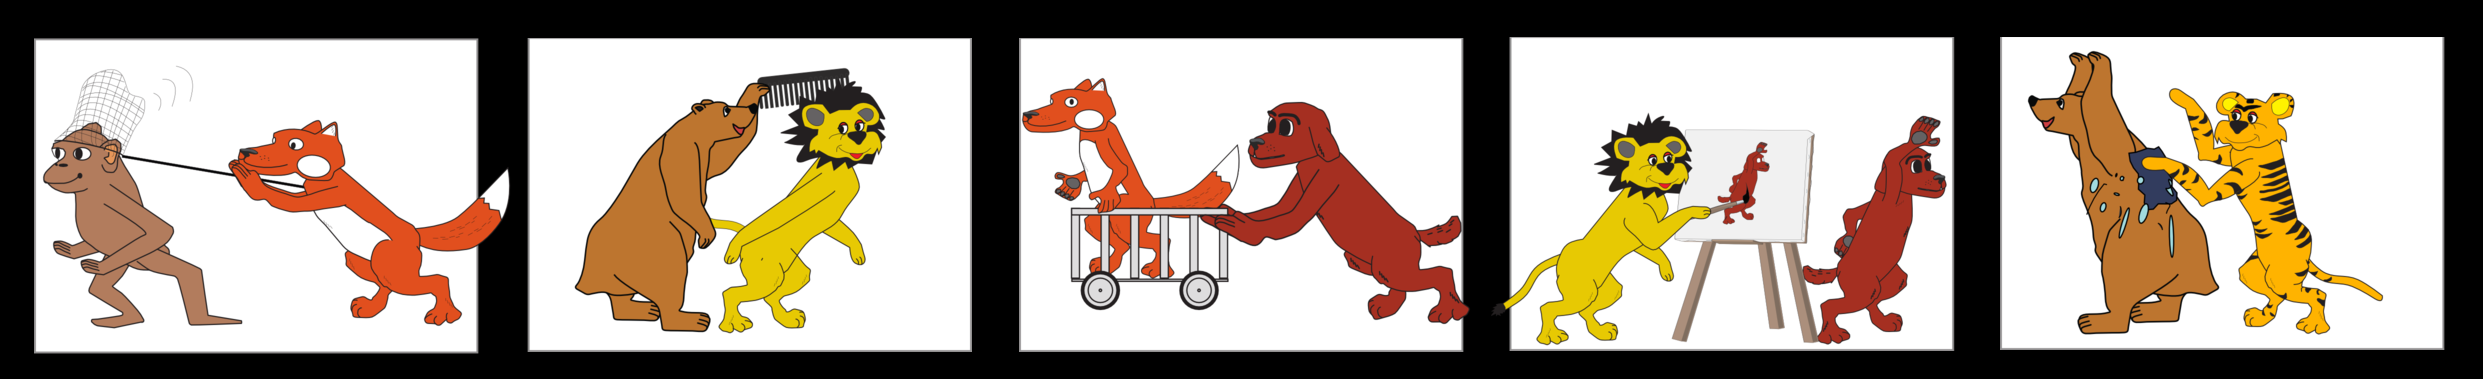
\includegraphics[width=0.99\textwidth]{pics/3_1_activities}
\caption{\label{3.1.activities} Illustrations of all five animals performing their social activities. From left to right: catching, combing, pushing, painting and washing}
\end{center}
\end{figure}

\paragraph{Trial feedback}
Immediately after each response, an icon appeared below one of the two displayed animal pairs.
The presented side was determined by the subject's response.
In the case of the skip button, the icon appeared at the same height as the others, but in the middle of the screen.
A green checkmark, a diagonal red cross and a yellow skip symbol signified a correct response, an incorrect response and an invalid trial, respectively.
The trial feedback screen was presented for a random interval between 400ms and 800ms.

\begin{figure}[h]
\begin{center}
\vspace{7mm}
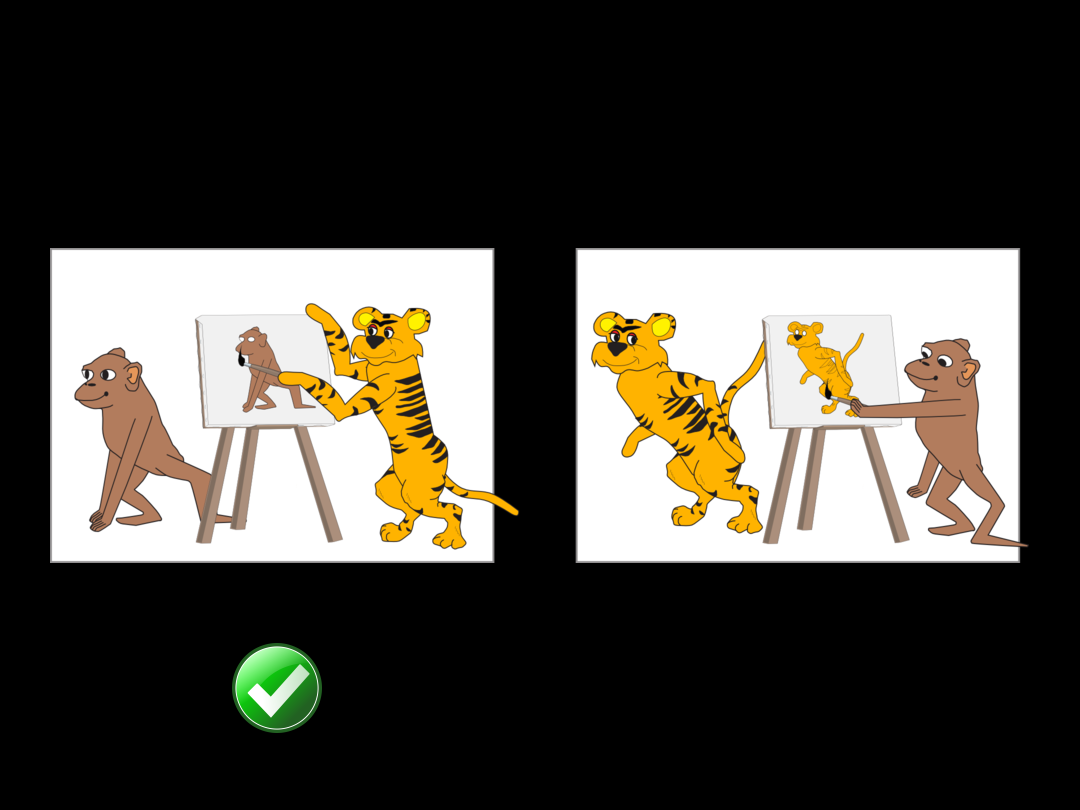
\includegraphics[width=0.5\textwidth]{pics/3_1_feedback}
\caption{\label{3.1.feedback} The visual feedback to a correct response.}
\end{center}
\end{figure}

\paragraph{Cluster feedback}
In this experiment, there was an obvious tradeoff between speed and accuracy.
To encourage a high level of attention and a high number of usable trials, two bar graphs visualized performance speed and accuracy (see Fig. \ref{3.1.clusterfeedback}).
In order to maximize the amount of usable trials for further analysis, the visualization valued accuracy much more than response time (see Fig. \ref{3.1.feedbackGraphs}).

\begin{figure}[h]
\begin{center}
\vspace{7mm}
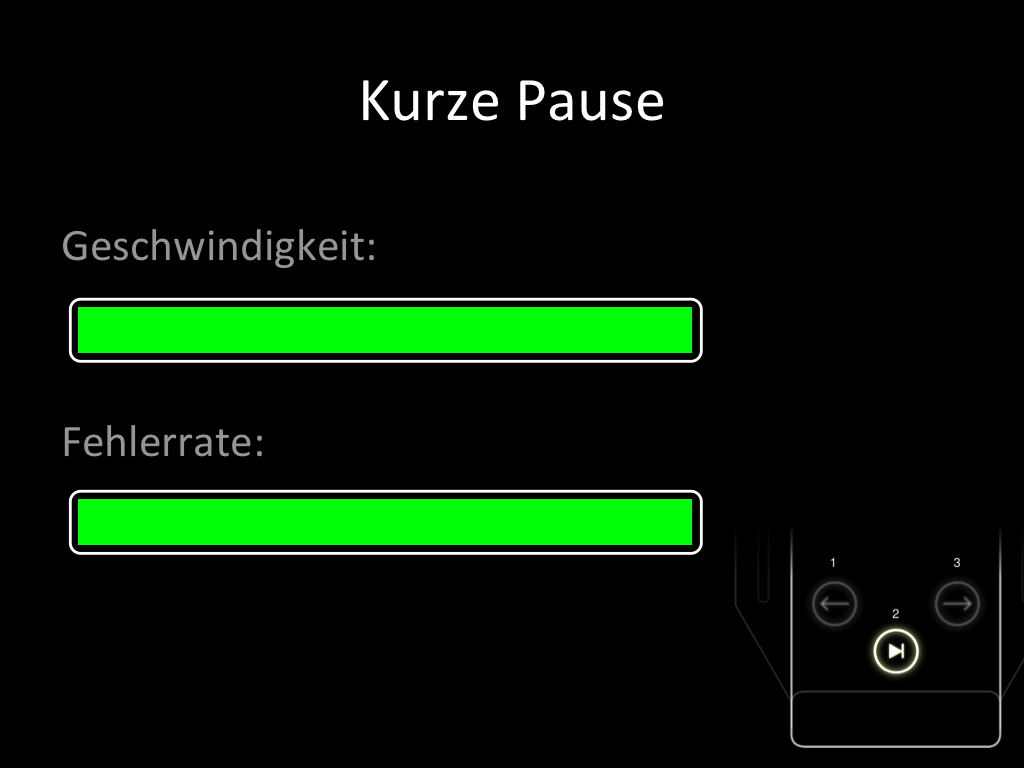
\includegraphics[width=0.5\textwidth]{pics/3_1_clusterfeedback}
\caption{\label{3.1.clusterfeedback} An ideal cluster feedback screen that appears after completing 19 trials. Upper bar: speed, lower bar: accuracy. Bottom right: indicator to  press the skip button to advance}
\end{center}
\end{figure}

\begin{figure}[h]
\begin{center}
\vspace{7mm}
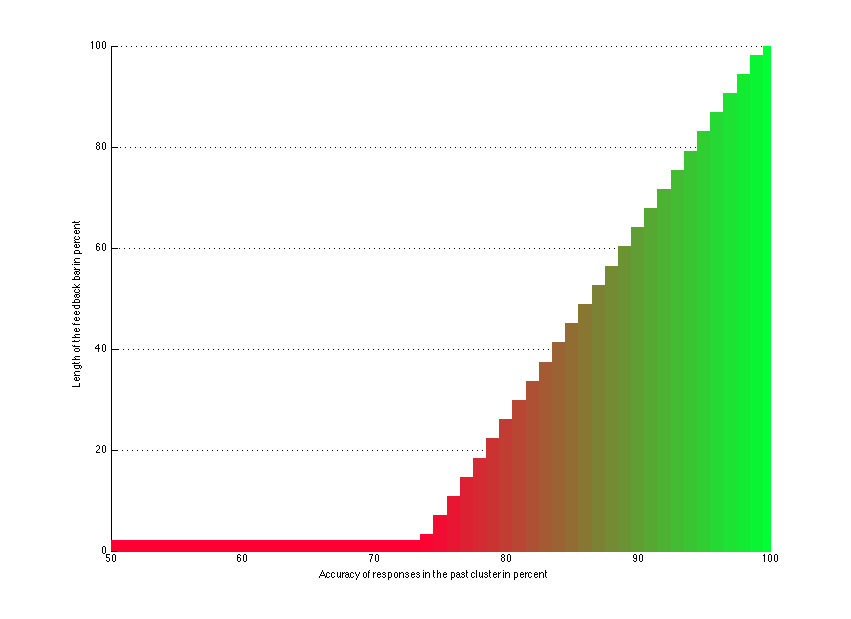
\includegraphics[width=0.45\textwidth]{pics/3_1_feedbackGraphAccuracy}
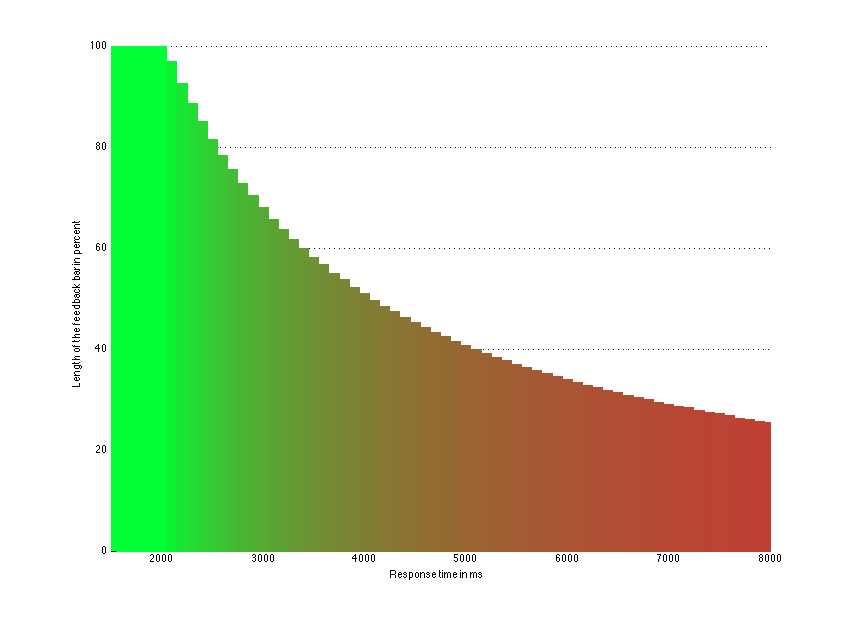
\includegraphics[width=0.45\textwidth]{pics/3_1_feedbackGraphRT}
\caption{\label{3.1.feedbackGraphs} Relation between performance and displayed feedback bars. Performance (left: RA, right: RT) is drawn along the X-axis, and length of the bars in \% is drawn along the Y-Axis.}
\end{center}
\end{figure}

\subsection{Auditory stimuli}\label{3.1.stimuli.auditory}

\paragraph{Sentence content}
Each pair of images was presented with a spoken question.
The question format fit well with the stimulus-response paradigm, and allowed the sentences to be identical until the conditional article ("'den"' or "'der"') appeared.
Syntactically, the sentences used an equal number of subject-relative and object-relative clauses.
In order to minimize confounding effects, these two conditions were designed to show as little auditory distinction as possible.
The structure of the final sentences is displayed in table \ref{3.1.sentences}.

\begin{table}[htb]
\vspace{5mm}
\begin{center}
\begin{tabular}{c|cccccccc}
Original & Wo & ist & das & Tier, & das & der & Tiger & malt?\\
Translated & Where & is & the & animal$_{OBJ}$, & which & the$_{NOM}$ & tiger$_{SUBJ}$ & paints?\\
Word index & 1 & 2 & 3 & 4 & 5 & 6 & 7 & 8
\end{tabular}
\caption{\label{3.1.sentences} Example stimulus sentence. Top: original spelling in German. Middle: Literal translation in English. Bottom: Word index within the sentence. NOM: Nominative case.}
\end{center}
\end{table}

\paragraph{Tutorial sentences}
During the pilot study, children often assumed that the every sentence was a subject-relative construction, miscategorizing "'den"' for "'der"'.
Tutorial sentences made the two animal nouns explicit, so that all sentences were structured in the format "'Where is the monkey that is caught by the dog?"'.
While this setup was creating strong auditory differences, it was easier to comprehend.
If the children didn't notice the difference by the eighth tutorial trial, the research assistant repeated the question with an exaggerated "'den"' pronounciation.

\paragraph{Audio format}
Sentences were spoken by a professional female native speaker in an uni\-so\-nous and moderately child-directed prosody.
Recording and playback was performed at a sampling rate of 44100Hz with one channel.
Loudness of each sentence was normalized.
Overall loudness was adjusted to 50db above each subject's individual hearing threshold.

\paragraph{Trial feedback}
Immediately after each response, one of two short sounds played.
The sounds were extracted from Microsoft Windows XP.
The "'external device plugged in"' icon (two bell sounds in ascending tone) and the "'external device removed"' icon (two bell sounds in descending tone) represented correct and incorrect responses, respectively.
No sound was played after the skip button.

\subsection{Experimental setup}
The participants were seated on a comfortable chair, inside a shielded, dimly-lit cabin.
Visual and auditory stimuli were produced by a computer running Presentation (version 14.0) at 60Hz refresh rate and 1024x768 resolution.
Video signal was routed through a video splitter MSV1235 into a Panasonic PT-D7700 projector.
Audio signals were generated by a Soundblaster Audigy 2 ZS [SB0350].
An audio amplifier (Compumedics, Hamburg, Germany) drove a pair of TIP-300 loudspeakers (Nicolet, Biomedical Madison, WI, U.S.A.).
Sound was routed through a pair of plastic tubes (50cm length, approx. delay of 1.6ms)
Sound arrived in the subjects' ears via ER3-14A/B earplugs (Etymotic Research Inc., Elk Grove Village IL, U.S.A.).

